%\subsection{Intégration }

Reprenant les travaux menés depuis quelques années à Montpellier et à Penang en Malaisie par Didier Schwab, nous avons réimplanté l'ensemble des outils permettants la fabrication et l'exploitation de vecteurs conceptuels (Blexisma 3 : Base LEXicale Sémantique Multi-Agent) en Java. Cela se traduit par la création de plus de 300 classes et interfaces disponible sous licence LGPL (Licence publique générale limitée GNU)\footnote{\url{http://ligforge.imag.fr/projects/blexisma/}}.

Plusieurs expériences sont en cours, toutes utilisent comme ressource un grand graphe lexical construit à partir de Wiktionary\footnote{\url{http://www.wiktionary.org/}}. 

\begin{itemize}

\item une première, de type émergence, calcule des vecteurs du français. Un service Web a été mis en place et est exploité par notre partenaire \textit{Ghanni} pour calculer des vecteurs conceptuels décrivant des textes compagnons de leur vidéos. L'anglais et l'allemand sont en phase d'intégration (voir figure \ref{emergence-videosense})


\begin{figure}[h!]
  \centering{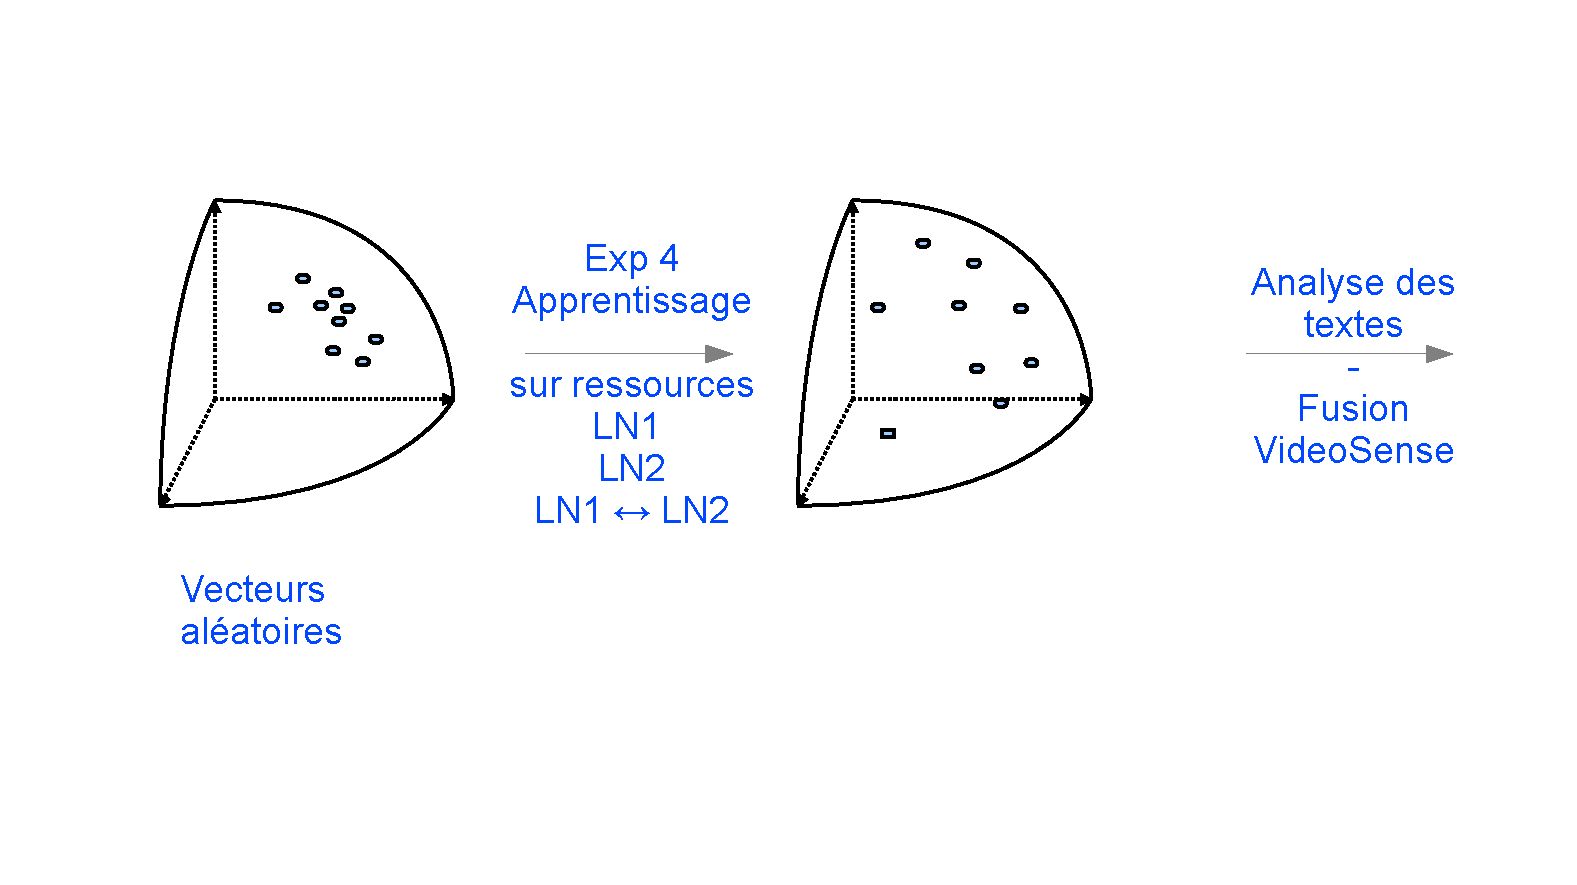
\includegraphics[width=18cm]{3_Experiences/img/experience-emergence}}
  %\vskip -3cm
\caption{Émergence des vecteurs dans VideoSense. Dans cette expérience, le français, l'anglais et l'allemand sont plongés dans un seul espace vectoriel. Les vecteurs conceptuels sont appris grâce aux informations issus de wiktionnary  : définitions et liens de traduction entre les langues}
\label{emergence-videosense}
\end{figure}

\item une seconde, qui aura plusieurs variantes, utilise elle une hiérarchie pour chaque langue. Les noyaux sont en phase de constitution, celui du français, le plus avancé en est environ à 40\% (voir figure \ref{hierarchies-videosense}).


\begin{figure}[h!]
  \centering{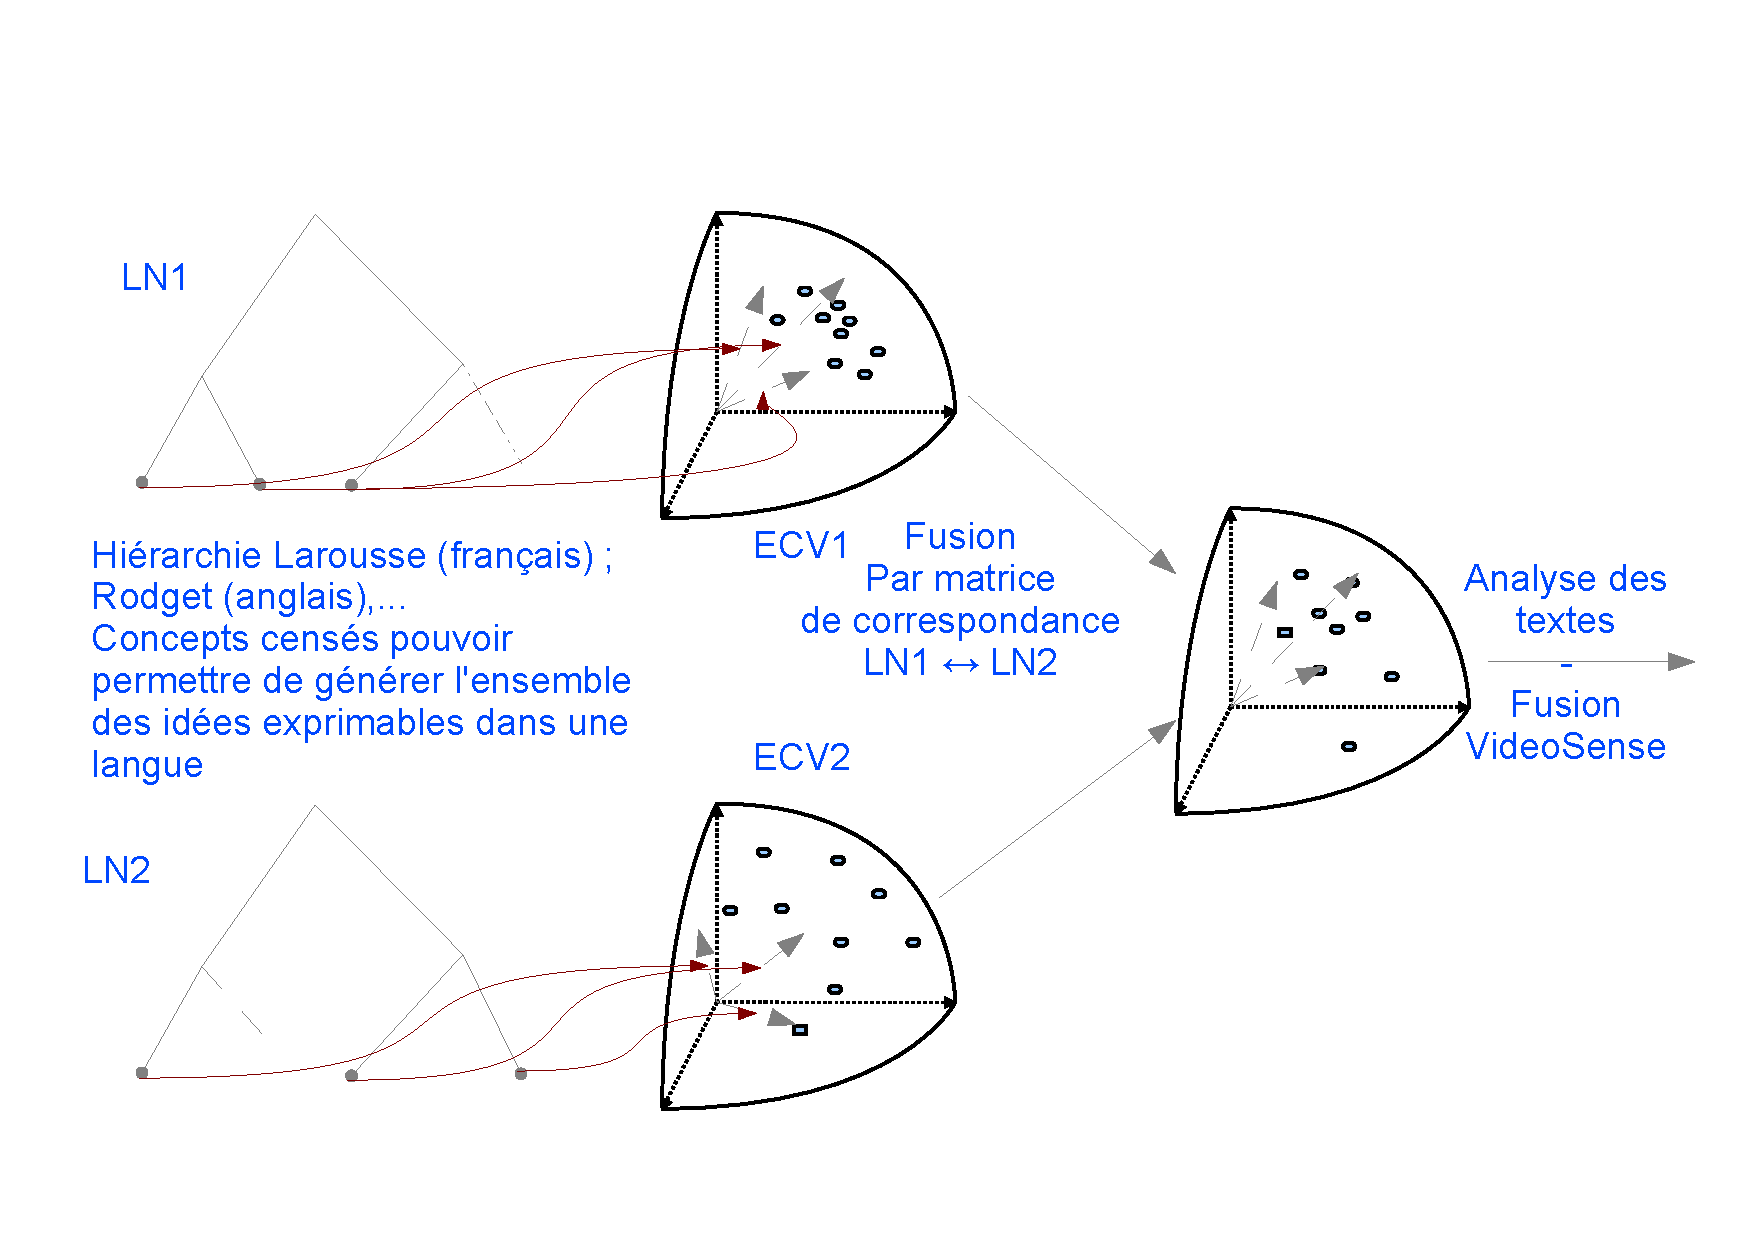
\includegraphics[width=18cm]{3_Experiences/img/Experience-hierarchies}}
\caption{Vecteurs construits à partir de hiérarchies dans VideoSense. Dans cette expérience, une hiérarchie est associée à chaque langue. La projection des langues dans un même espace vectoriel se fait grâce à une matrice de correspondance calculée semi-automatiquement à partir des hiérarchies.}
%  \vskip -3cm
\label{hierarchies-videosense}
\end{figure}

\end{itemize}

